\begin{figure}[htb!]
    \centering
    \caption{Relationship between log rents and the minimum wage measures, 
             sample of affected ZIP code-months}
    \label{fig:non_parametric}
    
    \begin{minipage}{.95\textwidth} \centering
        Panel A: Raw data
        \vspace{1mm}
    \end{minipage}
    \begin{subfigure}{0.5\textwidth}
        \caption*{Residence MW}
        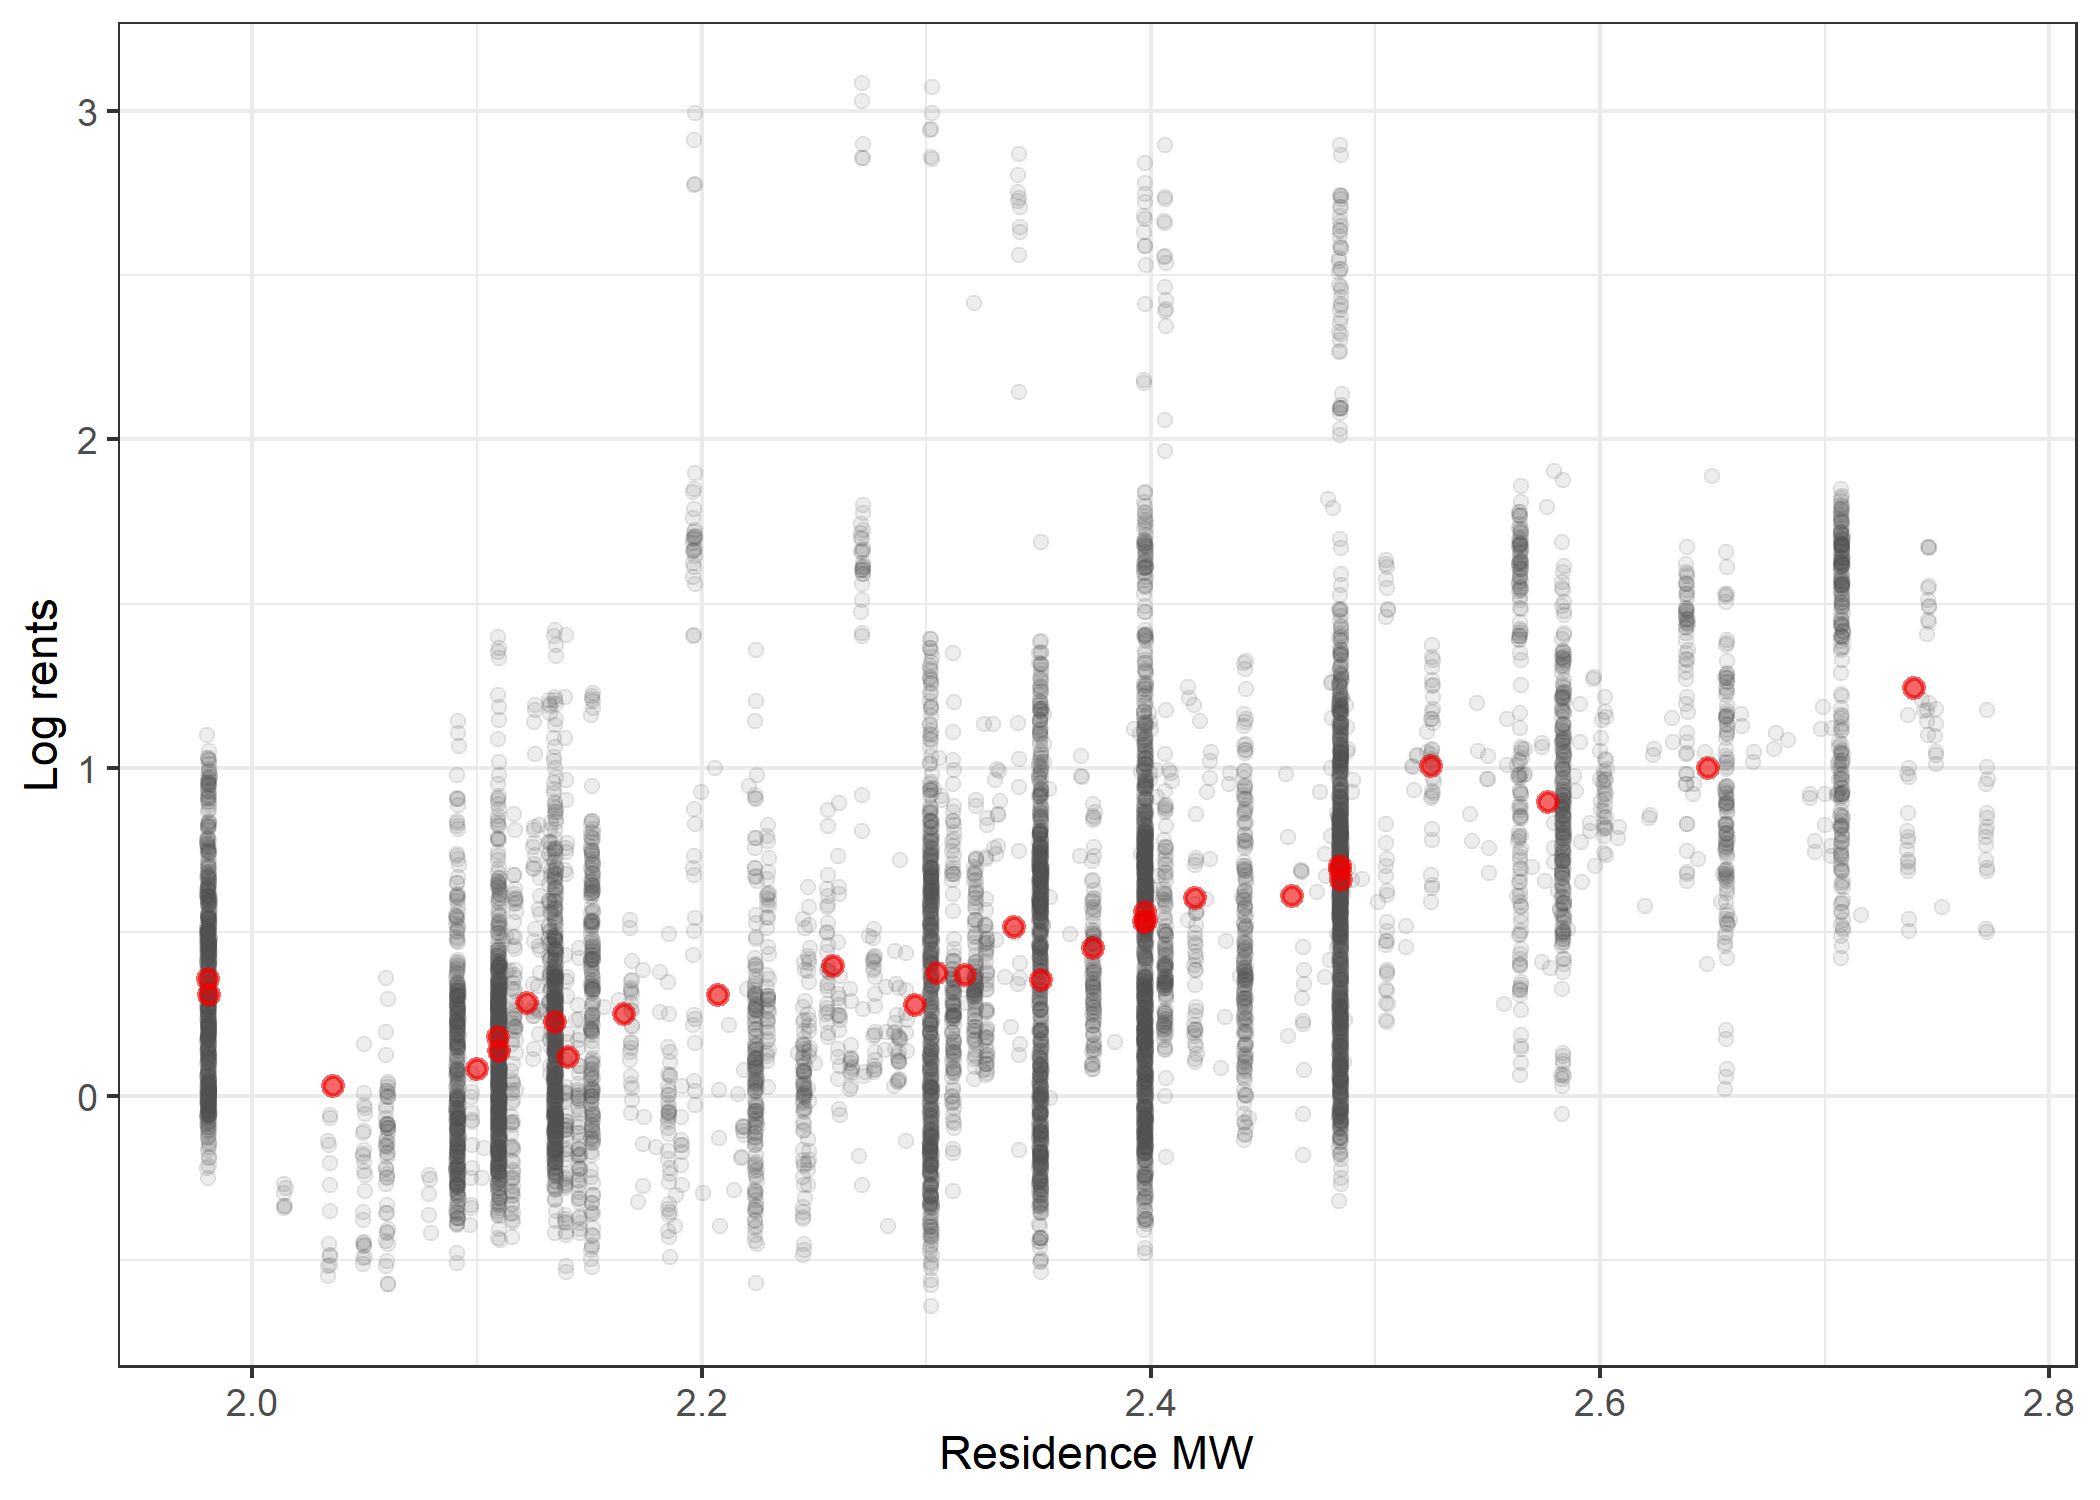
\includegraphics[width = 1\textwidth]{non_parametric/output/cbsa_month_mw_res}
    \end{subfigure}%
    \begin{subfigure}{0.5\textwidth}
        \caption*{Workplace MW}
        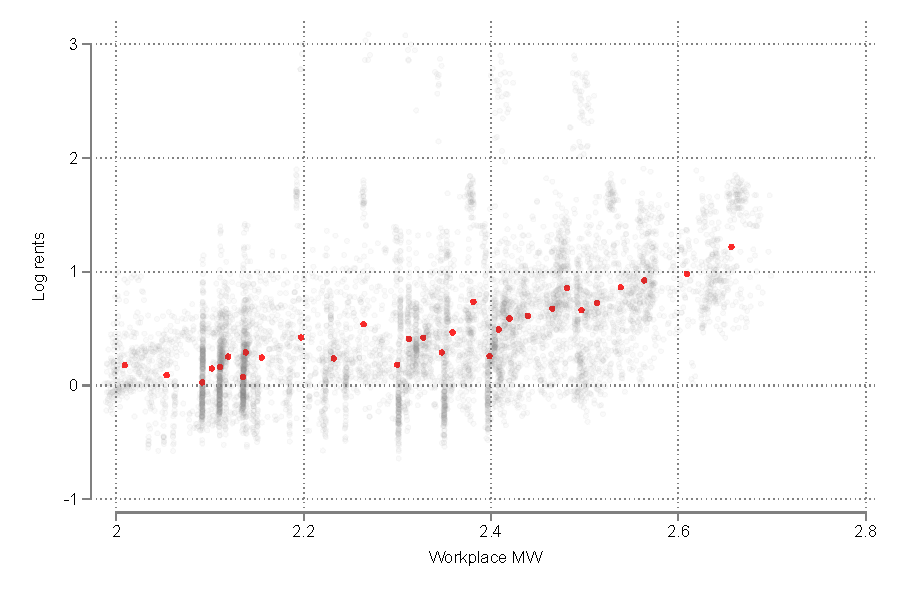
\includegraphics[width = 1\textwidth]{non_parametric/output/cbsa_month_mw_wkp}
    \end{subfigure}\\

    \vspace{2mm}
    \begin{minipage}{.95\textwidth} \centering
        Panel B: Conditional on ZIP code FE and the other MW measure
        \vspace{1mm}
    \end{minipage}
    \begin{subfigure}{0.5\textwidth}
        \caption*{Residence MW}
        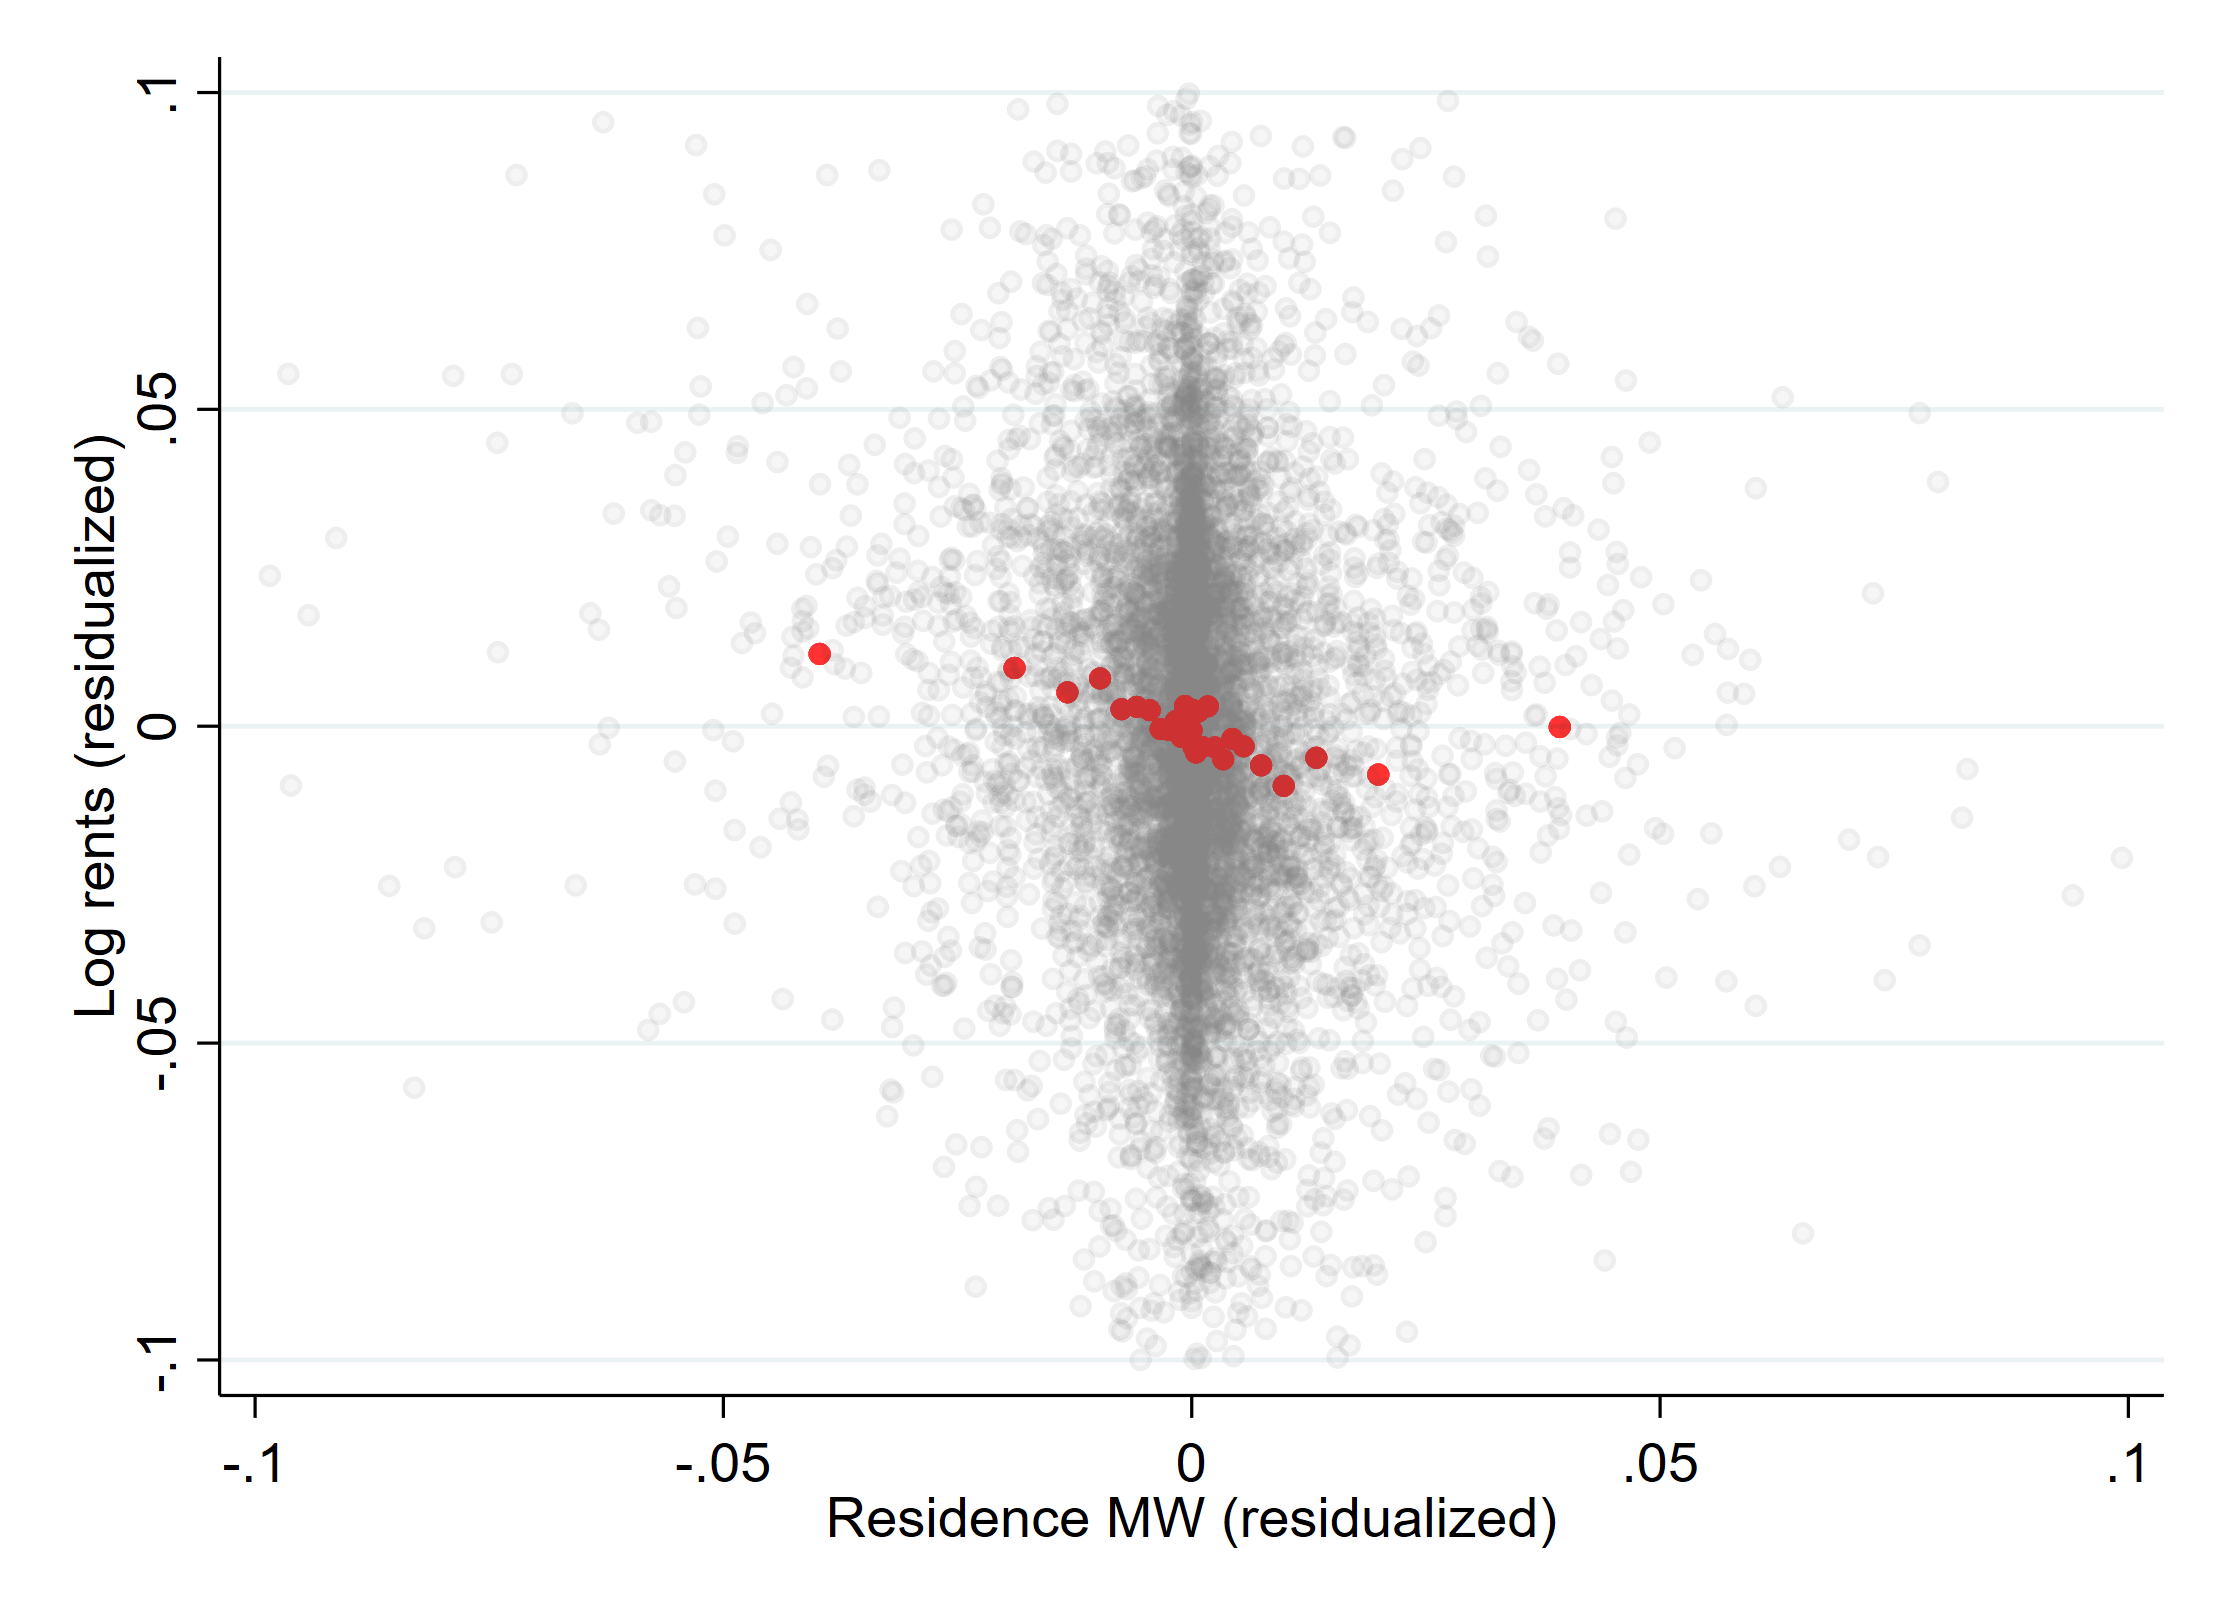
\includegraphics[width = 1\textwidth]{non_parametric/output/cbsa_month_mw_res_resid_mw_wkp_dec}
    \end{subfigure}%
    \begin{subfigure}{0.5\textwidth}
        \caption*{Workplace MW}
        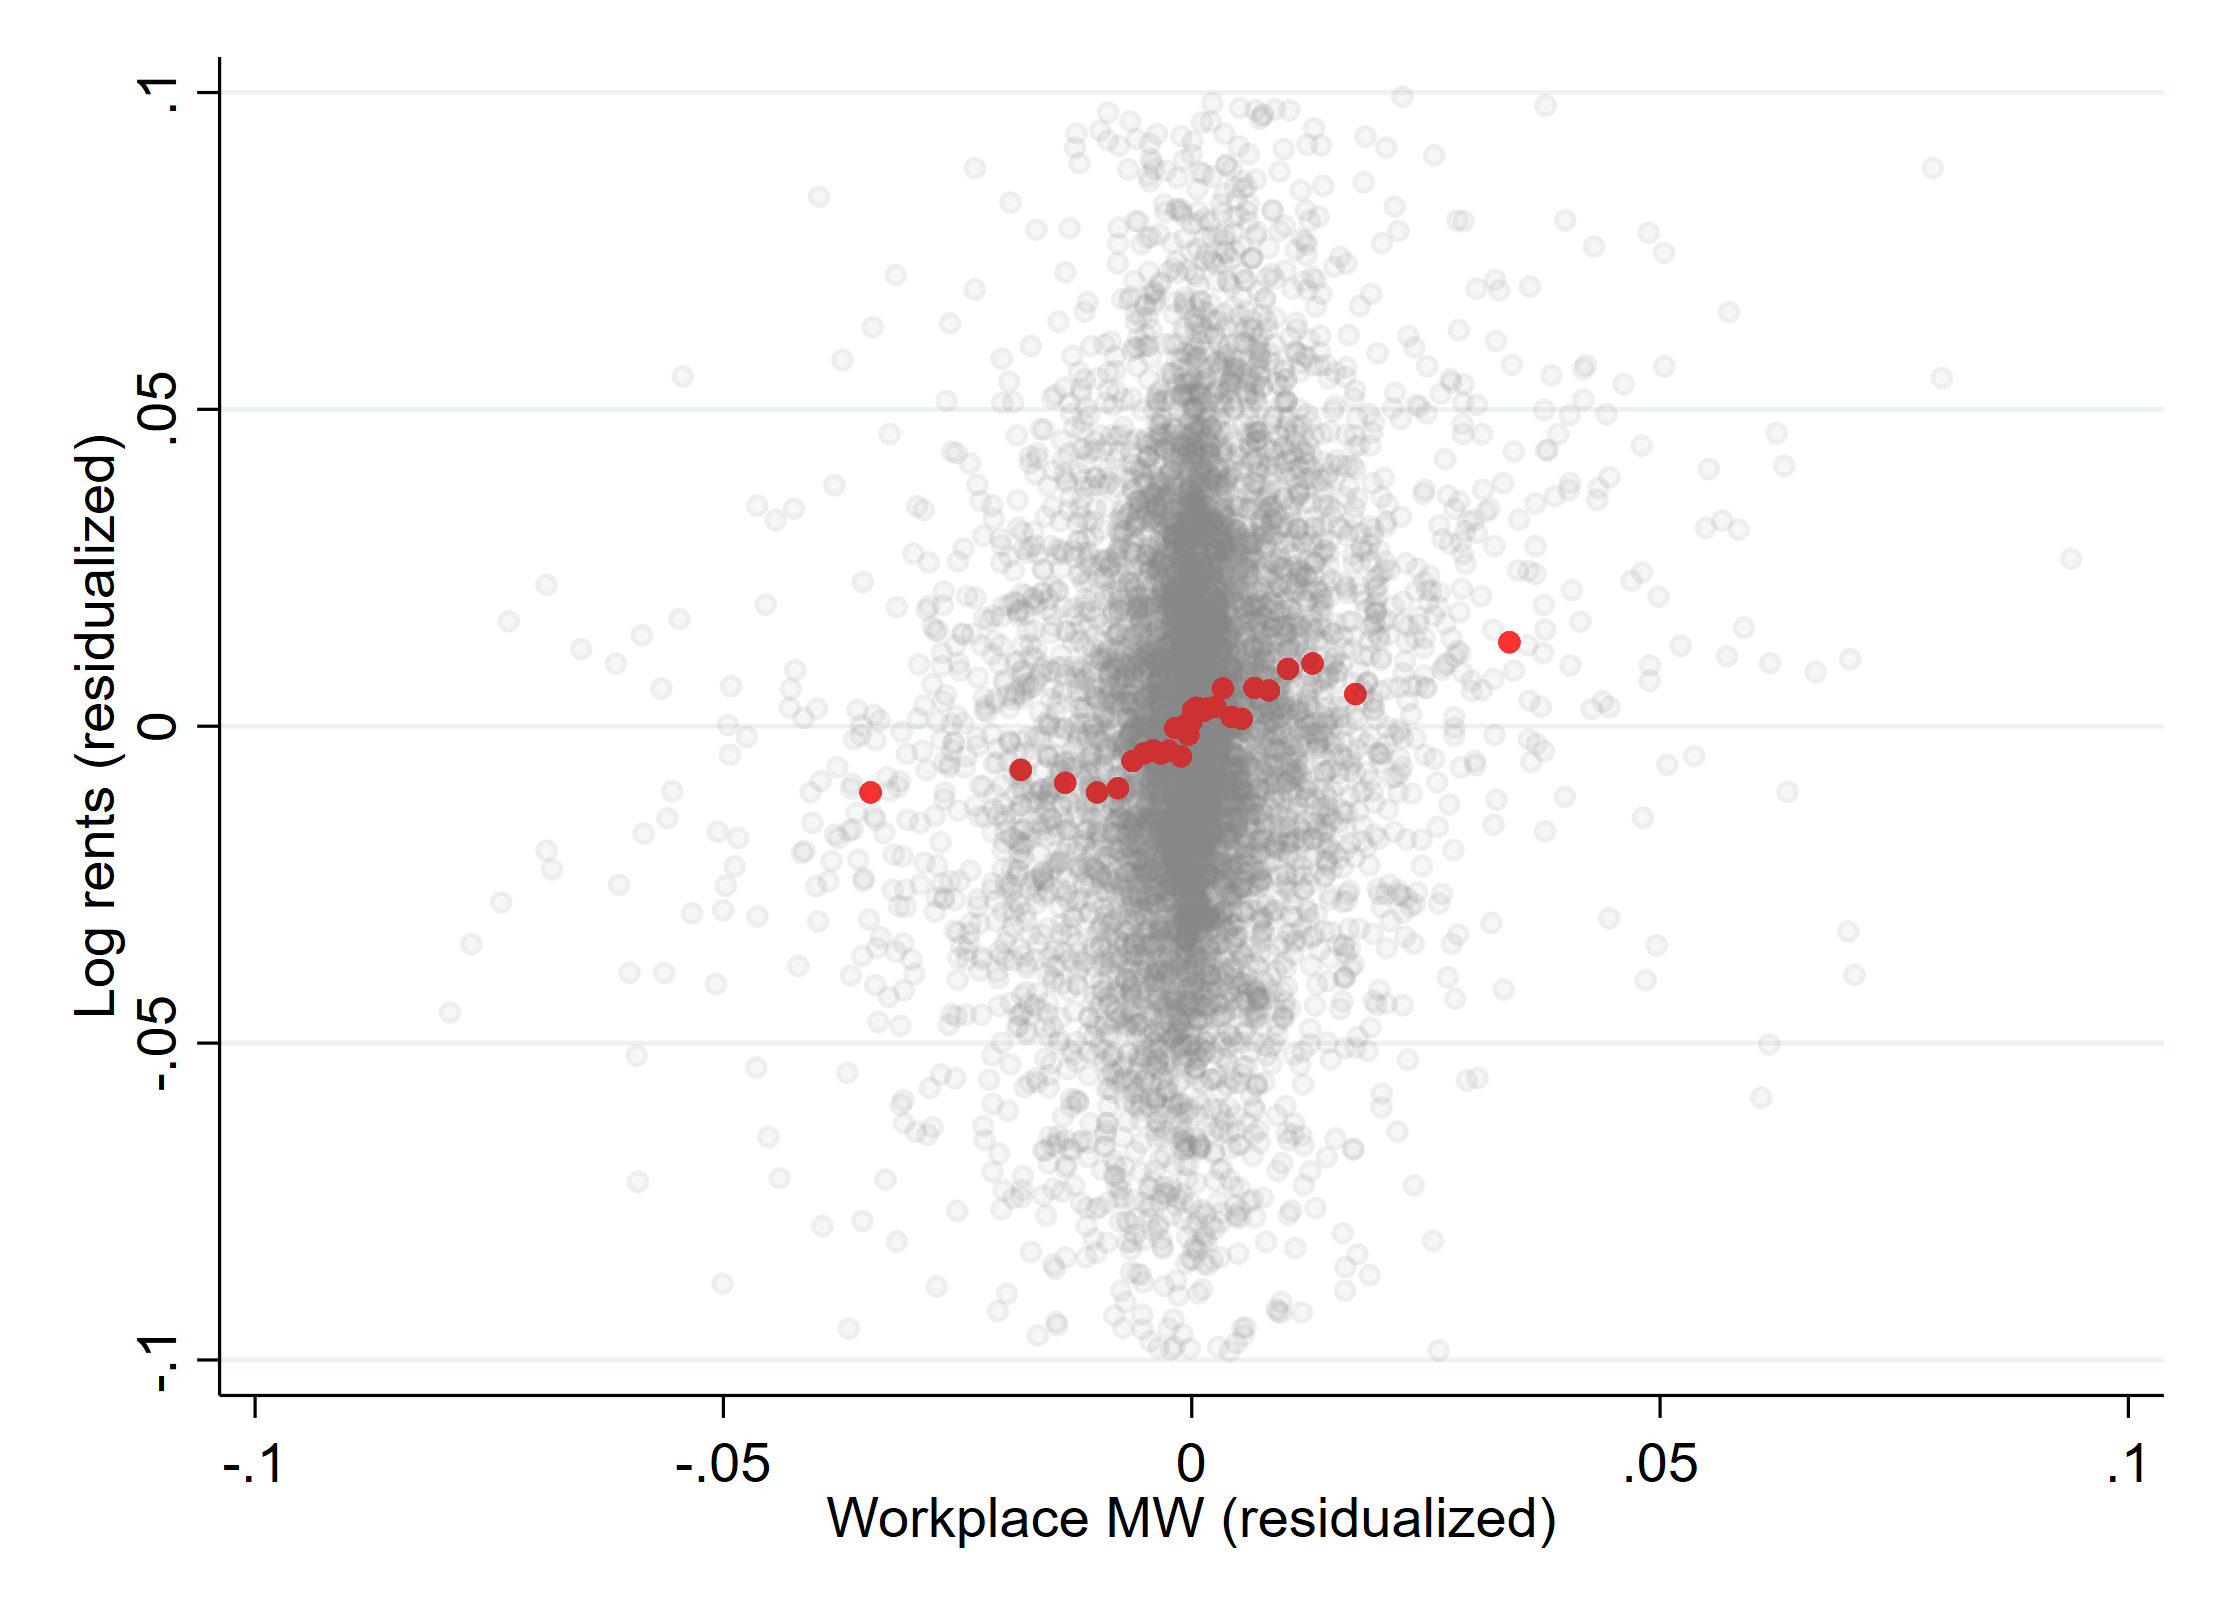
\includegraphics[width = 1\textwidth]{non_parametric/output/cbsa_month_mw_wkp_resid_mw_res_dec}
    \end{subfigure}

    \begin{minipage}{.95\textwidth} \footnotesize
        \vspace{3mm}
        Notes:
        Data are from Zillow and LODES.
        The plot shows the unconditional and conditional relationship between 
        log rents and the MW measures.
        The sample is composed of ZIP code-month observations located in CBSAs 
        where there was some statutory MW increase in the month of interest. 
        The rents variable correspond to log rents per square foot in the SFCC 
        category in Zillow.
        The workplace MW measure is constructed using commuting data from the 
        closest prior year.
        Panel A shows the raw relationship between log rents and workplace 
        and residence MW levels.
        Panel B shows the same relationship using residuals from regressions 
        on ZIP code indicators and 100 indicators of the other MW measure.
        Red dots correspond to 30 equally-sized bins of the $x$-axis variable.
        Gray dots correspond to all data points in Panel A, and only those 
        data points that fall within the range of the plot axes in Panel B.
    \end{minipage}
\end{figure}
